%
% File coling2014.tex
%
% Contact: jwagner@computing.dcu.ie
%%
%% Based on the style files for ACL-2014, which were, in turn,
%% Based on the style files for ACL-2013, which were, in turn,
%% Based on the style files for ACL-2012, which were, in turn,
%% based on the style files for ACL-2011, which were, in turn, 
%% based on the style files for ACL-2010, which were, in turn, 
%% based on the style files for ACL-IJCNLP-2009, which were, in turn,
%% based on the style files for EACL-2009 and IJCNLP-2008...

%% Based on the style files for EACL 2006 by 
%%e.agirre@ehu.es or Sergi.Balari@uab.es
%% and that of ACL 08 by Joakim Nivre and Noah Smith

\documentclass[11pt, a4paper]{article}
\usepackage{coling2014}
\usepackage{times}
\usepackage{url}
\usepackage{latexsym}
\usepackage{tipa}
\usepackage{graphicx}
%\usepackage{setspace}
%\usepackage{array}

% Lexicon/grammar entries
\usepackage{float}
\floatstyle{ruled}
\newfloat{entry}{thp}{lop}
\floatname{entry}{Entry}

% Ethiopic
\usepackage[english]{babel}
\usepackage{ethiop}
\newcommand{\eth}{\selectlanguage{ethiop}}

\selectlanguage{english}

%\setlength\titlebox{5cm}

% You can expand the titlebox if you need extra space
% to show all the authors. Please do not make the titlebox
% smaller than 5cm (the original size); we will check this
% in the camera-ready version and ask you to change it back.

\title{Minimal Dependency Grammar for Machine Translation}

\author{
%  Michael Gasser \\
%  School of Informatics and Computing \\
%  Indiana University \\
%  Bloomington, IN, USA \\
%  {\tt gasser@indiana.edu} \\\And
%  Alex Rudnick \\
%  School of Informatics and Computing \\
%  Indiana University \\
%  Bloomington, IN, USA \\
%  {\tt alexr@indiana.edu} \\
  }

\date{}

\begin{document}
\selectlanguage{english}
\maketitle
\begin{abstract}
This paper introduces Hiiktuu,
an ongoing project to develop a framework and a set
of tools for the creation of rudimentary bilingual lexicon-grammars for machine translation
into and out of under-resourced languages.
The basic units in Hiiktuu, called \textbf{groups}, are headed multi-item sequences.
In addition to wordforms, groups may contain lexemes, syntactic-semantic categories,
and grammatical features.
Each group is associated with one or more translations, each of which is a group in a target
language.
During translation, constraint satisfaction is used to select a set of source-language groups
for the input sentence and to sequence the words in the associated target-language
groups.

\end{abstract}

\section{Introduction}
\label{intro}

%
% The following footnote without marker is needed for the camera-ready
% version of the paper.
% Comment out the instructions (first text) and uncomment the 8 lines
% under "final paper" for your variant of English.
% 
\blfootnote{
    %
    % for review submission
    %
%    \hspace{-0.65cm}  % space normally used by the marker
%    Place licence statement here for the camera-ready version, see
%    Section~\ref{licence} of the instructions for preparing a
%    manuscript.
    %
    % % final paper: en-uk version (to license, a licence)
    %
    % \hspace{-0.65cm}  % space normally used by the marker
    % This work is licensed under a Creative Commons 
    % Attribution 4.0 International Licence.
    % Page numbers and proceedings footer are added by
    % the organisers.
    % Licence details:
    % \url{http://creativecommons.org/licenses/by/4.0/}
    % 
    % % final paper: en-us version (to licence, a license)
    
     \hspace{-0.65cm}  % space normally used by the marker
     This work is licenced under a Creative Commons 
     Attribution 4.0 International License.
%     Page numbers and proceedings footer are added by
%     the organizers.
     License details:
     \url{http://creativecommons.org/licenses/by/4.0/}
}

For the majority of the world's languages we lack
adequate resources to make use of the machine learning techniques that
have become the standard for modern computational linguistics.
Languages with inadequate resources include not only those with few
speakers, many of them endangered, but also a number of Asian and African languages with tens of
millions of speakers, such as Telugu, Burmese, Oromo, and Hausa.
For machine translation (MT) and computer-assisted translation (CAT),
the lack is even more serious because what is
required for machine learning is sentence-aligned translations.

For these reasons, work on many such languages will continue to
consist in large part in the writing of computational grammars and
lexica by people.
Because such work normally requires significant training and is
notoriously time-consuming, there is a need for tools to permit
researchers and language technology users to ``get off the ground''
with these languages, that is, to create rudimentary grammars and lexica that
will support basic applications and facilitate the language documentation process.

We focus on MT and CAT because a lack of linguistic resources correlates with a lack of written material, and
we would like to develop tools to aid human translators in translating documents into these languages.
Our long-term goal is a system that allows users with little or no linguistic experience
to write bilingual lexicon-grammars
for low-resource languages that can also be updated on the basis of corpora,
when these are available, and that can be easily integrated into a CAT system.

In this paper we describe the initial steps in developing Hiiktuu,\footnote{\textit{Hiiktuu} is the Oromo
word for a (female) translator.} a lexical-grammatical framework for MT and CAT.
Although our focus is on the language pairs Spanish-Guarani and Amharic-Oromo, we illustrate
Hiiktuu with examples from English-Spanish.

\section{Lexica and grammars}

\subsection{Phrasal lexica}
\label{subsect:phrase}

The idea of treating phrases rather than individual words as the basic units of a language
goes back at least to the proposal of a Phrasal Lexicon by Becker \shortcite{becker}.
In recent years, the idea has gained currency within the related frameworks of Construction Grammar \cite{steels}
and Frame Semantics \cite{fillmoreFS} as well as in phrase-based statistical machine translation (PBSMT).
Arguments in favor of phrasal units are often framed in terms of the ubiquity of idiomaticity, that is, departure
from strict compositionality.
Seen another way, phrasal units address the ubiquity of lexical ambiguity.
If a verb's interpretation depends on its object or subject, then it may make more sense to treat the combination
of the verb and particular objects or subjects as units in their own right.

Arguments based on idiomaticity and ambiguity are semantic, but they extend naturally to translation.
If the meaning of a source-language phrase fails to be the strict combination of the meanings
of the words in the phrase, then it is unlikely that the translation of the phrase will be the
combination of the translations of the source-language words.
Adding lexical context to an ambiguous noun or verb can sometimes permit an MT
system to select the appropriate translation.

\subsection{A simple phrasal lexicon}
\label{subsect:lexicon}

The basic lexical entries of Hiiktuu are multi-word units called \textbf{groups}.
Each group represents a catena \cite{osborneetal12}.
Catenae go beyond constituents (phrases), including all combinations of elements that are continuous
in the vertical dimension within a dependency tree.
For example, in the sentence \textit{I gave her a piece of my mind}, \{\textit{I, gave}\} and \{\textit{gave, her, piece}\}
are among the catenae but not the constituents of the sentence.

A catena has a head, and each Hiiktuu group must also have a head, which indexes the group within the lexicon.
A group's entry also specifies translations to groups in one or more other languages.
For each translation, the group's entry gives an \textbf{alignment}, representing inter-group correspondences between
elements, as in the phrase tables of PBSMT.
Entry~\ref{entry:end} shows a simple group entry of
this sort.\footnote{We serialize Hiiktuu lexical with YAML (\url{http://www.yaml.org/})}
The English group \textit{the end of the world} with head \textit{end} has as its Spanish translation
the group \textit{el fin del mundo} (which has its own entry in the Spanish lexicon).
In the alignment, each word other than the fourth word (\textit{the}) in the English group is associated with the position
of a word in the Spanish group.

\begin{entry}
%\begin{spacing}{.85}
\small
\begin{verbatim}
end:
  - words: [the, end, of, the, world]
    spa:
    - [el_fin_del_mundo, {align: [1,2,3,0,4]}]
\end{verbatim}
\normalsize
%\end{spacing}
\caption{Group entry for \textit{the end of the world} and its Spanish translation}
\label{entry:end}
\end{entry}

\subsection{The lexicon-grammar tradeoff}
\label{subsect:lexgram}

A rudimentary lexicon with entries of this sort is simple
in two senses: a user with no formal knowledge of linguistics can add entries in a
straightforward manner, and the resulting entries are
easily understood.
Such a lexicon permits the translation of sentences that are combinations
of the wordforms in the group entries, as long as group order is preserved across
the languages and there are no constraints between groups that would affect the form
of the target-language words.
However, such a lexicon permits no
{\em generalization} to combinations of wordforms that are not explicit in the lexicon.
It would require a group entry for every reasonably possible combination of
wordforms.
%Even for language pairs with enormous available bitext corpora,
%SMT researchers have discovered the need to incorporate some syntax in their systems.

At the other extreme from this simple lexicon is a full-blown grammar that is driven by
the traditional linguistic concern
%--- one might even say obsession --- 
with parsimony:
every possible generalization must be ``captured''.
Although it has the advantage of compactness and of reflecting general principles
of linguistic structure, such a grammar is difficult
to write, to debug, and to understand, requiring significant knowledge of linguistics.
%As we have seen, abstract word-based grammars also miss the information that is inherent
%in words in context.

In the Hiiktuu project, the goal is a range of possibilities along the continuum from
purely lexical (and phrasal) to syntactic/grammatical, with the emphasis on ease of entry
creation and interpretation.

\subsection{Lexemes}
\label{subsect:lexeme}

We can achieve significant generalization over simple groups consisting of wordforms by
permitting lexemes in groups.
As an example, consider the English group \textit{passV the buck}, where \textit{passV} is
the verb lexeme \textit{pass}.
In order to make such a group usable, the lexicon also requires \textbf{form} entries,
giving the lexeme roots as well as grammatical features for specific wordforms.
Some of these, along with the group entry, are shown in Entry~\ref{entry:pass}.

\begin{entry}
%\begin{spacing}{.85}
\small
\begin{verbatim}
groups:
  passV:
  - words: [passV, the, buck]
    spa:
      - [escurrir_el_bulto,
         {align: [1,2,3], agr: [{tns: tmp, prs: prs, num: num}, 0, 0]}]
forms:
  pass:
  - root: passV, features: {prs: 1, tns: prs}
  - root: passV, features: {prs: 3, num: plr, tns: prs}
  - root: passN, features: {num: sng}
  passes:
    root: passV, features: {prs: 3, num: sng, tns: prs}
  passed:
    root: passV, features: {tns: pst}
\end{verbatim}
\normalsize
%\end{spacing}
\caption{Group entry for \textit{pass the buck} and three form entries}
\label{entry:pass}
\end{entry}

Because this entry accommodates multiple sequences of English wordforms,
we need to map these onto appropriate target-language sequences.
This is accomplished through pairs of agreement features
for the lexeme, constraining the corresponding target language form to agree with the source
form on those features.
In the example, the
head \textit{passV} and its translation in the Spanish group agree on
tense and \textit{tiempo}, person and \textit{persona}, and number and \textit{n\'{u}mero} features.
For example, if this group is selected in the translation of the sentence \textit{Carl passes the buck},
the head of the corresponding Spanish group will be constrained to be
third person singular present tense (\textit{tiempo}):
\textit{Carl \textbf{escurre} el bulto}.

\subsection{Lexical/grammatical categories}
\label{subsect:cats}

Another simple way to generalize across groups is to introduce syntactic or semantic categories.
Consider the English expression \textit{give somebody a piece of one's mind}.
We can generalize across specific word sequences such as \textit{gave me a piece of his mind}
and \textit{gave them a piece of my mind} by replacing the specific wordforms in positions
2 and 6 in the group with categories that include the wordforms that can fill those positions.
This requires the forms dictionary to record the categories that wordforms belong to.
Entry~\ref{entry:mind} shows how this appears in the lexicon.
Category names are preceded by \$.

\begin{entry}
\small
\begin{verbatim}
groups:
  giveV:
  - words: [giveV, $sbd, a, piece, of, $sbds, mind]
    agr: [[1, 6, {prs: prs, num: num}]]
  my:
  - words: [my]
  mayor:
  - words: [the, mayor]
forms:
  my: [{cats: [$sbds]}]
  mayor: [{cats: [$sbd]}]
\end{verbatim}
\normalsize
\caption{Three group entries and two associated form entries}
\label{entry:mind}
\end{entry}

Because group positions that are filled by categories do not specify a surface form,
during parsing and generation of sentences they must be merged with other groups that match
the category and do specify a form.
For example, to parse or translate the sentence \textit{I gave the mayor a piece of my mind} requires
that positions 2 and 6 in the group \textit{giveV\_$sbd\_a\_piece\_of\_$sbds\_mind} be
filled by the heads of the groups \textit{the\_mayor} and \textit{my}.
This \textbf{node merging} process is illustrated in Figure~\ref{fig:mind}.

\begin{figure}[ht]
\begin{center}
  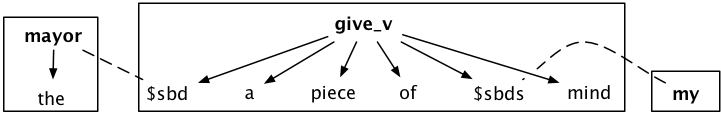
\includegraphics{mind}
\caption{Merging of three groups in \textit{gave the mayor a piece of my mind}}
\label{fig:mind}
\end{center}
\end{figure}

This group illustrates another requirement of some groups containing categories.
In \textit{give somebody a piece of one's mind}, the possessive adjective in the place of
\textit{one's} must agree with the subject of the sentence.
Since the group contains no subject, we constrain it to agree with the person and number
of the verb.
Thus the entry for this group also contains an agreement attribute specifying that
the the sixth element must agree with the first on person and number features.

\section{Constraint satisfaction and translation}
\label{sect:cs}

Translation in Hiiktuu takes place in three phases: analysis, transfer, and realization.
Analysis of the source-language sentence begins with a lexical lookup of the wordforms in the forms dictionary for
the source language.\footnote{In future versions
of the system, it will be possible to call a morphological analyzer on the input forms at
this stage.}
The words or lexemes resulting from this first pass are then used to look up candidate groups in the
groups dictionary.
Next the system assigns a set of groups to the input sentence.
A successful group assignment satisfies several constraints: (1)~each word in the input sentence
is assigned to zero, one, or (in the case of node merging) two group elements.
(2)~Each element in a selected group is assigned to one word in the sentence.
(3)~For each selected group, within-group agreement restrictions are satisfied.
(4)~For each category element in a selected group, it is merged with a non-category element in another
selected group (see the two examples in Figure~\ref{fig:mind}).
Analysis is a robust process; some words in the input sentence may end up unassigned to any group.

Analysis is implemented in the form of constraint satisfaction, making use of insights
from the Extensive Dependency Grammar framework (XDG) \cite{debusmann}.
Although considerable source-sentence ambiguity is eliminated because groups
incorporate context, ambiguity is still possible, particularly for figurative expressions
that also have a literal interpretation.
In this case, the constraint satisfaction process undertakes a search through the space of possible group
assignments, creating an analysis for each successful assignment.

During the transfer phase, a source-language group assignment is converted to an assignment of target-language
groups.
In this process some target-language items are assigned grammatical features on the basis of agreement constraints.
For example, in the translation of the English sentence \textit{the mayor passes the buck},
the Spanish verb that is the head of the group \textit{escurrir\_el\_bulto} would be
assigned the tense (\textit{tiempo}), person and number features \texttt{tmp=prs, prs=3, num=1}: \textit{escurre}.
A source-language group may have more than one translation.
The transfer phase creates a separate target-language group assignment for each combination of translations of the
source-language groups.

During the realization phase, for each target-language group assignment,
surface forms are generated based on the lexemes and grammatical features that resulted from
the transfer phase.
In the current version of the system, this is accomplished through a dictionary that maps
lexemes and feature sets to surface forms.\footnote{In future versions
of the system, it will be possible to call a morphological generator at
this stage.}
Finally, target-language words are sequenced in a way that satisfies word-order
conditions in target-language groups.
The sequencing process is implemented with constraint satisfaction.

\section{Related work}
\label{sect:related}

Our goals are similar to those of the Apertium \cite{apertium} project.
As with Apertium, we are developing open-source, rule-based systems for MT, and
we work within the framework of relatively shallow, chunking grammars.
We differ mainly in our willingness to sacrifice linguistic coverage
to achieve our goals of flexibility, robustness, and transparency.
We accommodate a range of lexical-grammatical possibilities, from the completely
lexical on the one extreme to phrasal units consisting of a single lexeme and one or more syntactic/semantic
categories on the other, and we are not so concerned that Hiiktuu grammars will accept many ungrammatical source-language
sentences or even output ungrammatical (along with grammatical)
translations.

In terms of long-term goals, Hiiktuu also resembles the Expedition
project \cite{mcshane+nirenburg}, which makes use of knowledge acquisition
techniques and naive monolingual informants to develop
MT systems that translate low-resource languages into English.
Our project differs first, in assuming bilingual informants and second, in aiming to
develop systems that are unrestricted with respect to target language.
In fact we are more interested in MT systems with low-resource languages as target languages
because of the lack of documents in such languages.

Although Hiiktuu is not intended as a linguistic theory, it is worth
mentioning which theories it has the most in common with.
Like Construction Grammar \cite{steels} and Frame Semantics \cite{fillmoreFS},
it treats linguistic knowledge as essentially phrasal.
Like synchronous context-free grammar (SCFG) \cite{chiang}, it associates multi-word units in
two languages, aligning the elements of the units and representing word order within each.
Hiiktuu differs from SCFG in having nothing like rewrite rules or non-terminals.
Hiiktuu belongs to the family of dependency grammar (DG) theories because the heads of its
phrasal units are words or lexemes rather than non-terminals.
It shares most with those computational DG theories that rely on
constraint satisfaction \cite{bojar04,debusmann,foth+menzel,wang+harper}.
However, it remains an extremely primitive form of DG,
permitting only flat structures with unlabeled arcs and no relations between groups
other than through the merge operation described in \ref{subsect:cats}.
This means that complex grammatical phenomena such as long-distance dependencies and
word-order variability can only be captured through specific groups.

\section{Status of project, ongoing and future work}
\label{sect:status}

The code for Hiiktuu and a set of lexical-grammatical examples
are available at [\textit{URL omitted to preserve anonymity}]
under the GPL license.
To date, we have only tested the framework on a limited number of
translations using various language pairs.
In order to develop more complete lexicon-grammars for Amharic-Oromo and
Spanish-Guarani,
we are working on methods for automatically extracting groups from
dictionaries in various formats and from the limited bilingual data that
are available.
As a part of this work, it will be crucial to determine whether
it is simpler to extract Hiiktuu groups from data than to extract
grammars of other sorts, for example, SCFG.
We are also implementing a GUI that will allow naive bilingual users to
create Hiiktuu entries.
Again we will want to evaluate the framework with respect to the simplicity
of entry creation.
For the longer term, our goal is tools for the intelligent elicitation of lexical entries;
for example, when two entries resemble one another, users could be queried about the
value of collapsing them into a more abstract entry.

As far as the grammatical framework is concerned, 
the lack of dependencies between the heads of groups leaves the system
without the capacity to represent some agreement constraints, for example, agreement
between a verb+object group and the verb's subject,
or major constituent order differences between source and target language.\footnote{
The only way to implement such constraints in the current version of Hiiktuu is through
groups that incorporate, for example, subjects in verb-headed groups, as in
\textit{\$sbd kickV \$sth}.}
To alleviate this problem, we will be implementing
dependencies between group heads, much as in the
``interchunk module'' of Apertium.

%Finally, though we have not yet looked into the details,
%the theory's relative simplicity and flexibility should allow it to be converted
%to other more elaborate formalisms, for example, SCFG.

\section{Conclusions}
\label{sect:conclusions}

Relatively sophisticated computational grammars, parsers, and/or generators
exist for perhaps a dozen languages, and usable MT systems exist for
at most dozens of pairs of languages.
This leaves the great majority of languages and the communities who speak them
relatively even more disadvantaged than they were before the digital revolution.
What is called for are methods that can be quickly and easily deployed to
begin to record the grammars and lexica of these languages and to use these
tools for the benefit of the linguistic communities.
The Hiiktuu project is designed with these needs in mind.
Though far from achieving our ultimate goals, we have developed a simple, flexible, and robust
framework for bilingual lexicon-grammars and MT/CAT that we hope will be a starting
point for a large number of under-resourced languages.

\bibliographystyle{acl}
\bibliography{hltdi}

\end{document}
